\chapter{Introduction} \label{sectionIntroduction}

When building software systems, we have several areas of concern: cost, delivery timeline, quality, etc. The cost and time-to-market are often the two problems given the highest priority in a project. However, engineers must consider the software quality to preserve the system's longevity. Despite its importance, the code and architecture quality can be challenging to understand and measure.

The art of programming began as something very tedious and error prone, with programmers writing every step of a process in a machine language. As this was not a great way to grow the industry, languages were developed so that programmers could reduce the manual effort of their programming and also improve the quality of their work by allowing the machine itself to transform the high-level code into something executable and efficient. \cite{lehman:1980}

With the creation of programming languages, the ability to build systems and applications has become a skill that most anyone can learn. Open source project create communities of learning and advancement. However, all systems need structure and an investment of time. \todo{TODO: Improve this paragraph.}

When we think about projects, we can assume that as time goes on and changes and additions occur within a system's source code, the complexity of that system will grow. However, when we manage the code structure, we can keep the complexity in check, allowing systems to evolve. Developers can maintain this structure through simple steps like having readable code and more complex considerations, like how coupled and cohesive a system is.

One way to understand the quality around a system is to discuss its ``maintainability,'' the ease of receiving new features or resolving bugs. For example, developers may find that adjusting one area to add a new feature requires touching several other code areas in tightly coupled systems. Some code measuring systems provide a Maintainability Index (MI), a well-known quality measure. While the effectiveness in quantifying software quality is debated, many quality models include MI measurements \cite{vandeursen:2014}, \cite{adewumi:2016}. Adewumi et. al found that maintainability is measured by 55\% of the existing Open Source Software (OSS) quality models, making it the most common quality characteristic measured \cite{adewumi:2016}.

\begin{figure}[ht]
  \centerline{
      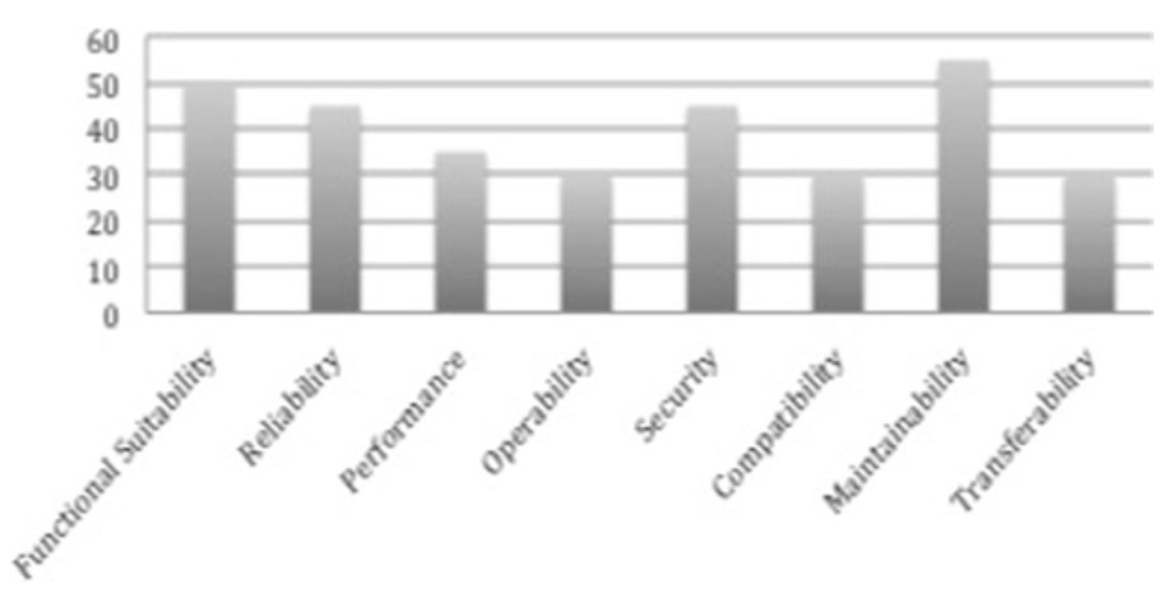
\includegraphics[width=0.7\columnwidth]{adewole_ProductQualityCharacteristics_in_OSS_quality_models.png}
  }
  \caption{Frequency distribution of ISO 25010 product quality characteristics in OSS quality models, as found by Adewumi et. al in 2016 \cite{adewumi:2016}.}
  \label{figFreqDistProductQualityModel}
\end{figure}

From ``Fig.~\ref{figFreqDistProductQualityModel}'', we can infer that maintainability is more important than functional stability. If the code is maintainable and accessible, missing features can be incorporated, but if it is difficult to read and understand and is not well documented, those missing features would be hard to implement \cite{adewumi:2016}.

Code smells are used extensively by practitioners to identify low-quality spots in the software system. These areas would need the teams' attention and are good candidates for refactoring. Rather than putting focus on building comprehensive models with all possible software characteristics, developers should instead focus on the essential characteristics: maintainability, usability, and maintenance capacity of a software community \cite{adewumi:2016}.

% \todo{TODO: Consider analogy of how Blockbuster did not evolve and eventually closed.}
